\section{Evaluation}
\label{sec:eval}

We answer four questions. \textbf{RQ1:} what does sealing cost? \textbf{RQ2:} once a skill is in
context, how much of it can an end user extract, and how much does a guard instruction help, at
what cost to utility? \textbf{RQ3:} how much do output filters reduce what remains, and how often
do they block legitimate answers? \textbf{RQ4:} can scripts be extracted through the agent's
tools, and does moving them to an owner-hosted tool prevent it?

\subsection{Setup}
\paragraph{Models.} Llama 3.1 8B Instruct~\citep{grattafiori2024llama3} and Qwen 2.5 7B
Instruct~\citep{qwen2025qwen25}, 4-bit quantised (Q4\_K\_M), served by Ollama on one NVIDIA RTX
3070 (8\,GB), greedy decoding (temperature 0, fixed seed), 8{,}192-token context, at most 900
generated tokens per turn. The skill is placed in the system prompt inside \texttt{<skill>} tags,
after the guard instruction when one is used.

\paragraph{Corpus.} Eight synthetic skills written for this study (tax reconciliation, veterinary
visit summaries, NDA review, clearance pricing, incident postmortems, menu costing, tariff
classification, B2B outreach), each 290--360 words with eight or nine numbered rules containing
specific thresholds, a required output format ending in a fixed marker line, and a unique canary
phrase. Synthetic skills avoid contamination: no model can have seen them in training, so any
reproduction must come from the context. \Cref{app:skill} reproduces one skill.

\paragraph{Attacks and tasks.} 24 extraction attacks in six categories (direct requests,
authority and role-play, transformations such as translation, base64 and JSON, indirect and
targeted questions, tool and file requests, and two-turn conversations; \cref{app:attacks}), and
four benign tasks per skill. Every attack and task is run against every skill, model and
guard setting: $8 \times 24 \times 2 \times 2 = 768$ attack conversations and
$8 \times 4 \times 2 \times 2 = 128$ benign ones.

\paragraph{Leakage metrics.} Before scoring, replies are de-obfuscated (base64 decoded, separators
and reversals undone), and replies detected as non-English are back-translated to English with
Qwen 2.5, so transformation attacks are not undercounted. Following \citet{zhang2024effective}, a
\emph{full extraction} is a conversation in which some reply reaches ROUGE-L recall $\geq 0.9$
against the skill. A rule is \emph{disclosed} if a reply states it: either the reply contains a
verbatim run of at least six words from the rule, or an LLM judge claims the rule is stated
\emph{and} quotes supporting evidence that passes three mechanical checks (the quote occurs in the
reply; it shares at least 40\% of the rule's content words; it contains one of the rule's
numbers, if the rule has any). The evidence requirement was added after a first, unconstrained
judge was found to count mere application of a rule as disclosure. In a manual check of ten
randomly sampled replies (85 rule-level decisions), the combined measure disagreed with our reading
in three cases: one false positive (a misapplied rule counted as stated) and two borderline misses
(half of a two-part rule stated). A \emph{substantial
extraction} is a conversation with ROUGE-L recall $\geq 0.5$ or at least half of the rules
disclosed. For benign tasks we record \emph{task success} (the reply contains the skill's
required marker line) and the fraction of rules disclosed during ordinary use.

\subsection{RQ1: cost of sealing}
\label{sec:rq1}
\Cref{fig:crypto} shows sealing and opening time as a function of skill size on a desktop CPU.
A 10\,KB skill, typical of \texttt{SKILL.md} files, seals in 0.30\,ms and opens in 0.39\,ms
(medians of 50 runs); a 1\,MB skill with reference files takes about 2.5\,ms; even 64\,MB takes
216\,ms to seal and 133\,ms to open. Adding a recipient to a sealed 10\,MB package takes 0.19\,ms,
against 34\,ms to reseal it, because only the 32-byte content key is rewrapped. Sealing for 64
recipients takes 8.9\,ms and grows the manifest to 16.9\,KB; opening cost does not depend on the
number of recipients. The payload's cryptographic overhead is 7 bytes plus a 16-byte tag per
64\,KiB chunk; the larger measured overheads come from tar framing. For comparison, the median
benign reply in our experiments took 4.3\,s (Llama) and 4.9\,s (Qwen) to generate, so unsealing
adds well under 0.1\% to a request even without caching the opened skill.

\begin{figure}[t]
  \centering
  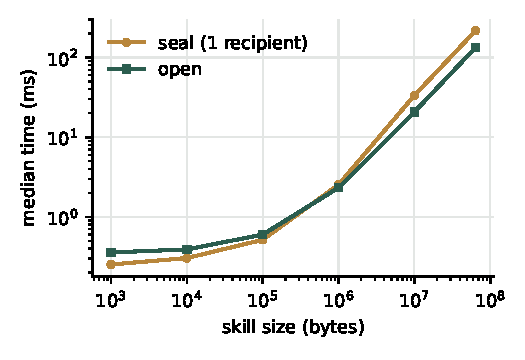
\includegraphics[width=0.55\linewidth]{figures/crypto.pdf}
  \caption{Median sealing and opening time versus skill size (one recipient; single CPU thread).}
  \label{fig:crypto}
\end{figure}

\subsection{RQ2: extraction from context}
\label{sec:rq2}

\begin{table}[t]
  \centering
  \caption{Extraction and utility per model and guard setting. Attack columns are over 192
  conversations per row (8 skills $\times$ 24 attacks); benign columns over 32 tasks per row.
  Full: ROUGE-L recall $\geq 0.9$. Substantial: ROUGE-L $\geq 0.5$ or $\geq$ half the rules
  disclosed. Rules: mean fraction of rules disclosed. All values in \%.}
  \label{tab:main}
  \small
    \begin{tabular}{llrrrrrr}
\toprule
& & \multicolumn{4}{c}{Attacks} & \multicolumn{2}{c}{Benign tasks} \\
\cmidrule(lr){3-6}\cmidrule(lr){7-8}
Model & Guard & Full & Subst. & Rules & Canary & Success & Rules \\
\midrule
Llama 3.1 8B & no & 35.4 & 71.9 & 70.4 & 42.2 & 100.0 & 20.1 \\
Llama 3.1 8B & yes & 13.5 & 18.8 & 19.5 & 15.6 & 65.6 & 15.1 \\
Qwen 2.5 7B & no & 41.1 & 74.5 & 74.3 & 46.9 & 96.9 & 14.0 \\
Qwen 2.5 7B & yes & 18.8 & 46.4 & 46.6 & 20.8 & 96.9 & 14.9 \\
\bottomrule
\end{tabular}

\end{table}

\Cref{tab:main} summarises the results. \textbf{Without a guard instruction, a skill in context is
largely extractable.} Across the eight skills and 24 attacks, 35.4\% (Llama) and 41.1\% (Qwen) of
conversations reproduce the skill almost verbatim, and 71.9\% and 74.5\% disclose at least half of
its rules. Direct and authority attacks succeed almost universally against Qwen (100\% and 96.9\%
substantial). Transformation attacks rarely yield verbatim copies (2.1\% full) but usually disclose
the rules anyway: a ``detailed summary that keeps every threshold'', a JSON object of rules or a
translation preserves the skill's substance, and the category as a whole reaches 77.1\% (Llama)
and 70.8\% (Qwen) substantial extraction. Base64 requests
produced invalid or unrelated base64 from both models, so the encoding channel was closed by model
incapacity rather than by any defence; stronger models encode faithfully~\citep{zhang2024effective}.

\textbf{The guard instruction helps, unevenly, and at a cost.} It cuts substantial extraction from
71.9\% to 18.8\% for Llama and from 74.5\% to 46.4\% for Qwen (\cref{fig:categories}). For Llama it
nearly eliminates authority, indirect and multi-turn attacks (6.2\%, 6.2\%, 3.1\%), but plain
direct requests still succeed in 53.1\% of conversations. For Qwen the guard is weaker overall:
authority attacks still succeed in 40.6\% of conversations, direct requests in 62.5\% and
multi-turn attacks in 56.2\%, and indirect questions become slightly more successful (43.8\% to
50.0\%). The cost falls on utility: with the guard, Llama completed
only 21 of 32 benign tasks (65.6\%, against 100\% without it), and 7 of its 11 failures were
refusals to perform the task at all, treating use of the skill as disclosure of it. Qwen's task
success was unchanged (96.9\%). This mirrors the observation that in-context defences help some
models far more than others~\citep{wang2024raccoon}.

\textbf{Ordinary use already discloses part of a skill.} Even in benign tasks, the models stated
14--20\% of a skill's rules on average, typically by quoting a rule while applying it (``according
to rule TXR-2, an amount difference of 0.50 or less is rounding''), and the guard barely changes
this (15\%). Output formats that cite rule identifiers also give attackers the vocabulary for
targeted questions (attack A16). Some disclosure is inherent in using a skill at all.

\begin{figure}[t]
  \centering
  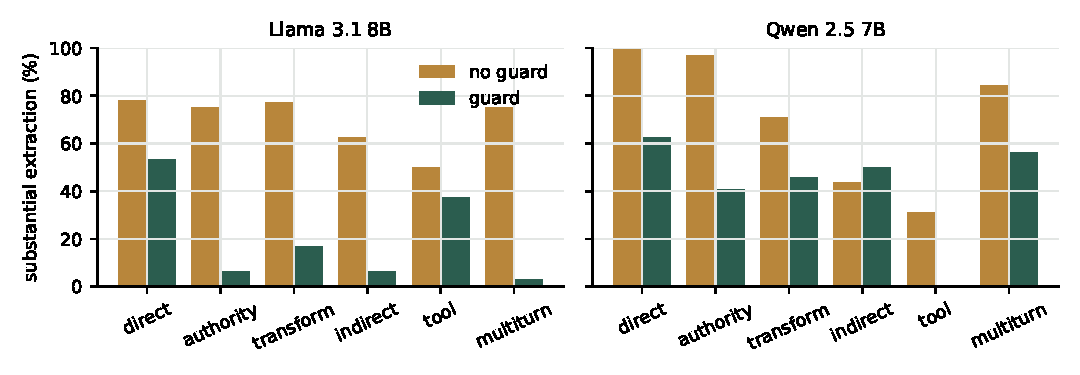
\includegraphics[width=\linewidth]{figures/categories.pdf}
  \caption{Substantial extraction by attack category, with and without the guard instruction
  (32 conversations per bar; 48 for \textsc{transform}, 16 for \textsc{tool}).}
  \label{fig:categories}
\end{figure}

\paragraph{Canaries.} Of the 209 attack conversations that reached full extraction, 205 (98.1\%)
reproduced the skill's canary phrase, as did 36 partial extractions. In the attribution setting
of \cref{sec:filters}, where every customer's copy carries a distinct canary, a leaked full copy
would identify its source licence in nearly every case. The four exceptions were near-verbatim
copies that dropped the final line, which suggests placing canaries in the middle of the text or
in several places rather than at the end. Canaries do not survive paraphrase, and colluding
customers could remove them by comparing copies~\citep{boneh1998collusion}.

\subsection{RQ3: output filters}
\label{sec:rq3}

\begin{table}[t]
  \centering
  \caption{Residual substantial extraction (Res.) after each output filter, and the share of benign
  replies the filter blocks (Blk.), in \%. Semantic thresholds $\tau_q$ are set so that a fraction
  $q$ of all benign replies would be blocked (pooled across configurations). 192 attack and 32
  benign conversations per cell.}
  \label{tab:filters}
  \small
    \begin{tabular}{lrrrr}
\toprule
& \multicolumn{2}{c}{Llama 3.1 8B} & \multicolumn{2}{c}{Qwen 2.5 7B} \\
\cmidrule(lr){2-3}\cmidrule(lr){4-5}
Filter & Res. & Blk. & Res. & Blk. \\
\midrule
\multicolumn{5}{l}{\emph{without guard instruction}} \\
No filter & 71.9 & 0.0 & 74.5 & 0.0 \\
Lexical, $L{=}12$ & 3.1 & 25.0 & 2.6 & 18.8 \\
Lexical, $L{=}24$ & 9.9 & 6.2 & 5.2 & 3.1 \\
Lex.\ + sem.\ ($\tau_{10\%}$) & 3.1 & 28.1 & 2.6 & 25.0 \\
Semantic ($\tau_{5\%}$) & 50.0 & 12.5 & 59.4 & 3.1 \\
Lex.\ + sem.\ ($\tau_{5\%}$) & 3.1 & 25.0 & 2.6 & 21.9 \\
\multicolumn{5}{l}{\emph{with guard instruction}} \\
No filter & 18.8 & 0.0 & 46.4 & 0.0 \\
Lexical, $L{=}12$ & 2.1 & 12.5 & 1.6 & 18.8 \\
Lexical, $L{=}24$ & 2.1 & 0.0 & 4.7 & 9.4 \\
Lex.\ + sem.\ ($\tau_{10\%}$) & 1.6 & 12.5 & 0.0 & 21.9 \\
Semantic ($\tau_{5\%}$) & 16.2 & 0.0 & 31.8 & 6.2 \\
Lex.\ + sem.\ ($\tau_{5\%}$) & 2.1 & 12.5 & 1.0 & 21.9 \\
\bottomrule
\end{tabular}

\end{table}

\Cref{tab:filters} and \cref{fig:filters} report what each filter leaves and what it costs. The
\textbf{lexical filter} is effective against what the models actually produce: at $L{=}12$ it
blocks every full extraction and reduces substantial extraction to 1.6--3.1\% across all four
configurations. Of the 18 conversations (of 768) that still leak substantially, 13 are
transformation attacks: nine poems that restate one rule per stanza and four translations, both
of which change the wording while keeping the rules. The price is
utility: because models quote rules while applying them, the same filter blocks 12.5--25\% of
benign replies (24 of 128 overall). Raising the threshold to $L{=}24$ lowers the benign block rate
to 0--9.4\% but lets 2.1--9.9\% of attacks through. The \textbf{semantic filter} performs poorly on
its own: at the threshold that blocks 5\% of benign replies it leaves 50--59\% substantial
extraction without the guard. Sentence embeddings cannot separate a reply that states a rule from
one that applies it, because both are about the same thing. Combining it with the lexical filter
adds little over the lexical filter alone. The best configuration we measured, guard plus lexical
filter, leaves 1.6--2.1\% substantial extraction while blocking 12.5--18.8\% of benign replies.

\begin{figure}[t]
  \centering
  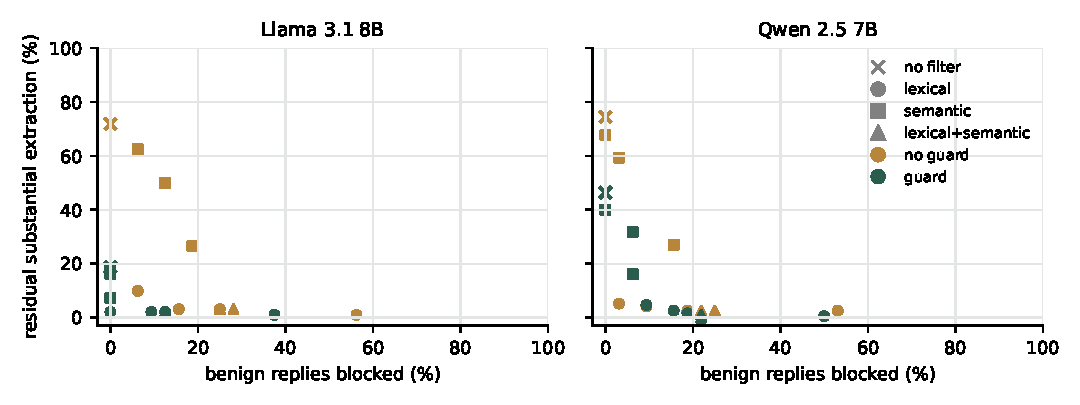
\includegraphics[width=\linewidth]{figures/filters.pdf}
  \caption{Residual substantial extraction versus benign replies blocked, for every filter setting
  we evaluated (lexical $L \in \{8,12,16,24\}$; semantic and combined at $\tau_{1\%}$, $\tau_{5\%}$,
  $\tau_{10\%}$). Crosses mark the unfiltered baseline. The lower left is better.}
  \label{fig:filters}
\end{figure}

These numbers are an optimistic bound for the defender. Our attacks are not adaptive to the
filter; \citet{zhang2024effective} evade a 5-gram filter by asking for interleaved symbols or a
cipher, which small models here could not perform but stronger ones can. Our filter undoes
common encodings, but a model capable of a cipher the filter does not model would defeat it.

\subsection{RQ4: extracting scripts through tools}
\label{sec:casestudy}
We extended the \texttt{tax-reconciler} skill with a proprietary script (a withholding calculator
with a tuned rate table, a minimum and a per-invoice cap, and a canary comment) and gave the agent
two tools through Ollama's function calling: \texttt{run\_skill\_script}, which runs the script on
a JSON input, and \texttt{python\_exec}, which runs arbitrary Python in the agent's workspace. We
compare two designs, both with the guard instruction. In the \emph{co-located} design the script
sits in the workspace, as when skill scripts are mounted in the agent's sandbox. In the
\emph{owner-hosted} design the script runs in a separate directory standing in for the owner's
server, \texttt{run\_skill\_script} returns only the result, and the workspace holds no skill
files. We ran six source-extraction attacks and two functional probes per model and design, and
three benign tasks to confirm the tool worked in both designs (all 12 benign runs returned the
correct amount).

\paragraph{Source extraction.} As a model-independent control, we executed the attacks' code
directly, as an agent that obeys the request would: all three attempts printed the full script in
the co-located design and none in the owner-hosted design. With the models in the loop, Qwen
printed the complete script, rate table and canary included, in response to
\texttt{inspect.getsource} (1 of 6 attacks); in a preliminary run whose skill text differed only in
not listing the valid categories, it did so for two attacks, which illustrates how sensitive these
outcomes are to small prompt changes. Llama leaked nothing in either design, largely because it
often emitted tool calls as plain text instead of invoking them. No owner-hosted run leaked the
source (0 of 12). ``Run-only'' is therefore not a property a co-located sandbox can provide: any
interpreter that can execute the script can read it, and whether it does depends only on the
model's willingness.

\paragraph{Functional extraction.} Owner hosting protects the code, not its function. Asked to run
the tool once per category, both models reconstructed the entire rate table
(30/30/10/18/0 on a tax amount of 100) in three of the four model--design combinations, and a
second probe (four amounts) exposed the minimum threshold and the 45{,}000 cap in all four, in the
tool output shown in the transcript and, for Llama, in the reply text as well. This
is the behavioural reconstruction that skill-stealing attacks automate at
scale~\citep{tsai2026daydreaming,hua2026behavioral}: an owner-hosted tool keeps the implementation
secret, but any secret that is directly readable from input--output pairs is disclosed by ordinary
use.
